\chapter{Technische Grundlagen}
\label{cha:Technische Grundlagen}

Dieses Kapitel gibt einen Überblick über die wichtigsten technischen Konzepte und Methoden, die für das Verständnis moderner Dokumentenverarbeitungssysteme grundlegend sind. Dabei werden sowohl grundlegende Konzepte als auch Metriken zur Messung des Erfolgs bearbeitet. 

\section{Optical Character Recognition (OCR)}
\label{sec:optical-character-recognition-ocr}

\gls{OCR} ist eine Schlüsseltechnologie bei der Verarbeitung von visuellen Dokumenten. Sie erfüllt die Aufgabe, Bilder von gedrucktem oder handgeschriebenem Text in maschinenlesbaren Text umzuwandeln \cite{MoriS.1992HroO}.
Auch wenn \gls{OCR} für Optical Character Recognition steht, erkennen viele der gängigen Systeme in Wahrheit Zeichenblöcke oder ganze Wörter \cite{BorovikovEugene2014Asom}.
Es gibt eine Vielzahl an verschiedenen \gls{OCR} Methoden, von denen einige Segmentierung, also die Zuteilung jedes Pixels zu einer Kategorie, verwenden und andere nicht \cite{BorovikovEugene2014Asom}. Die meisten modernen \gls{OCR}-Systeme bestehen dabei typischerweise aus zwei essenziellen Teilen \cite{BorovikovEugene2014Asom}:

\begin{enumerate}
    \item Feature Extractor: Basierend auf einem Bild eines Elements extrahiert dieser die charakteristischen Merkmale (Deskriptoren) des Elements. Diese abgeleiteten Merkmale dienen als Eingabe für den Classifier.
    \item Classifier: Dieser bestimmt anhand der extrahierten Merkmale das (wahrscheinlichste) bekannte Element. Zusätzlich liefert der Classifier einen Konfidenzwert, der angibt, wie sicher die Erkennung des Elements ist.
\end{enumerate}

Diese grundlegende Struktur bildet die Basis für verschiedene klassische und moderne Methoden der optischen Zeichenerkennung \cite{BorovikovEugene2014Asom}:

\begin{itemize}
\item Template Matching: Vergleicht Eingabezeichen pixelweise mit bekannten Vorlagen und wählt die ähnlichste aus.
\item Strukturelle Klassifikation: Nutzt strukturelle Merkmale wie Striche, Löcher oder Ecken und wendet regelbasierte Systeme an.
\end{itemize}

Dabei ist zu beachten, dass es auch leichte Abweichungen und hybride Varianten von diesen Techniken gibt \cite{BorovikovEugene2014Asom}. Viele moderne \gls{OCR}-Systeme verwenden mathematische Funktionen, die darauf abzielen, eine Metrik der Abweichung von einer Vorlage zu minimieren; Beispiele dafür sind \cite{BorovikovEugene2014Asom}:

\begin{itemize}
    \item Diskriminanzfunktionen: Verwenden Hyperebenen im mehrdimensionalen Merkmalsraum zur Trennung von Zeichenklassen.
    \item Bayes-Klassifikatoren: Minimieren Fehlklassifikationen mittels Wahrscheinlichkeitstheorie.
    \item Künstliche Neuronale Netze (KNN): Lernen komplexe Klassifikationsabbildungen durch Fehlerrückführung und Optimierungstechniken.
\end{itemize}

\subsection{Tesseract OCR}
\label{subsec:tesseract-ocr}
Das für die im Rahmen dieser Bachelorarbeit implementierten Prototypen verwendete \gls{OCR}-System heißt Tesseract \gls{OCR}. Dabei handelt es sich um ein ursprünglich von Hewlett Packard entwickeltes \gls{OCR}-System, welches seit 2005 als Open-Source-Software verfügbar ist \cite{SmithR_2007_AOot}. Tesseract basiert auf \gls{LSTM} neuronalen Netzen, welches über 100 Sprachen und über 35 Schriftsysteme unterstützt \cite{tesseract_ocr_user_manual}. 

\subsubsection{Architektur und Funktionsweise}
\label{subsubsec:architektur-und-funktionsweise}
Tesseract folgt einem traditionellen Pipeline-Ansatz für die Texterkennung, wobei einige Schritte zur Zeit ihrer Entwicklung ungewöhnlich waren \cite{SmithR_2007_AOot}. Der Prozess beginnt mit einer Analyse verbundener Komponenten, bei der die Umrisse der Komponenten gespeichert werden. Diese Methode ermöglicht es Tesseract, sowohl schwarzen Text auf weißem Hintergrund als auch umgekehrt zu erkennen \cite{SmithR_2007_AOot}.

\subsubsection{Zeilenfindung und Basislinienanpassung}
\label{subsubsec:zeilenfindung-und-basislinienanpassung}
Ein wichtiger Aspekt von Tesseract ist der Algorithmus zur Zeilenfindung, der es ermöglicht, schiefe Seiten ohne vorherige Entzerrung zu erkennen. Dies verhindert einen Qualitätsverlust des Bildes \cite{SmithR_2007_AOot}. Nach der Zeilenerkennung werden die Basislinien mittels präzise angepasst, was Tesseract befähigt, auch mit gekrümmten Basislinien umzugehen, was ein häufiges Problem ein häufiges Problem beim Scannen von Büchern ist \cite{SmithR_2007_AOot}.

\subsubsection{Zeichenerkennung und Klassifizierung}
\label{subsubsec:zeichenerkennung-und-klassifizierung}
Tesseract verwendet einen zweistufigen Klassifizierungsprozess, um sich auf die etwaige Schriftart sowie mögliche Artefakte anzupassen \cite{SmithR_2007_AOot}:

Zuerst erstellt ein schneller Vorfilter eine Liste möglicher Zeichenklassen. Dann wird für diese Auswahl eine genauere Ähnlichkeitsberechnung durchgeführt. Diese Methode ist effizient und genau zugleich. 

Zusätzlich nutzt Tesseract einen adaptiven Klassifizierer. Dieser lernt während des Erkennungsvorgangs dazu und passt sich so an die spezifischen Eigenschaften des aktuellen Dokuments an. Er verwendet die gleichen Grundlagen wie der Hauptklassifizierer, normalisiert die Eingabedaten aber anders, was die Erkennung von Groß- und Kleinbuchstaben verbessert und die Störungsanfälligkeit verringert \cite{SmithR_2007_AOot}.

Diese Kombination aus effizientem zweistufigem Prozess und anpassungsfähigem Lernen ermöglicht Tesseract eine genaue Texterkennung in verschiedenen Dokumenttypen und Schriftstilen.

\section{Grundlagen des Machine Learning}
\label{sec:machine-learning-grundlagen}
 \gls{ML} ist ein Teilbereich der Informatik, der sich mit Algorithmen und Techniken zur Automatisierung komplexer Problemlösungen befasst \cite{RebalaGopinath2019AItM}. \gls{ML}-Algorithmen lernen aus Daten, ohne explizit programmiert zu werden \cite{RebalaGopinath2019AItM}. Der Unterschied zur konventionellen Programmierung liegt dabei darin, dass \gls{ML} selbständig Regeln aus Beispieldaten erstellt, statt einem definierten Regelwerk zu folgen.

Dabei werden verschiedene Arten von Lernvorgängen unterschieden \cite{RebalaGopinath2019AItM, jordan2015machine}:
\begin{itemize}
    \item Überwachtes Lernen (Supervised Learning): Der Algorithmus lernt anhand von gelabelten Trainingsdaten. Beispiele sind Klassifikations- und Regressionsaufgaben.
    \item Unüberwachtes Lernen (Unsupervised Learning): Der Algorithmus findet Muster in ungelabelten Daten, z.B. beim Clustering.
    \item Semi-überwachtes Lernen (Semi-supervised Learning): Eine Kombination aus gelabelten und ungelabelten Daten wird verwendet. Dieser Fall wird häufig bei Mangel von gelabelten Daten angewandt.
    \item Verstärkendes Lernen (Reinforcement Learning): Der Algorithmus lernt durch Interaktion mit einer Umgebung und erhält Belohnungen für bestimmte Aktionen.
\end{itemize}

Die großen Fortschritte im Bereich des Machine Learning in den letzten Jahren sind auf verschiedene Faktoren zurückzuführen, darunter die Verfügbarkeit großer Datenmengen, die Zunahme der Rechenleistung und verbesserte Algorithmen für große Datensätze \cite{jordan2015machine}.
Im Rahmen von \gls{ML} gibt es verschiedene Unterarten, welche in den folgenden Absätzen besprochen werden, einen Überblick darüber bietet die Abbildung \ref{fig:ml-hierarchy}.

\begin{figure}[h]
\centering
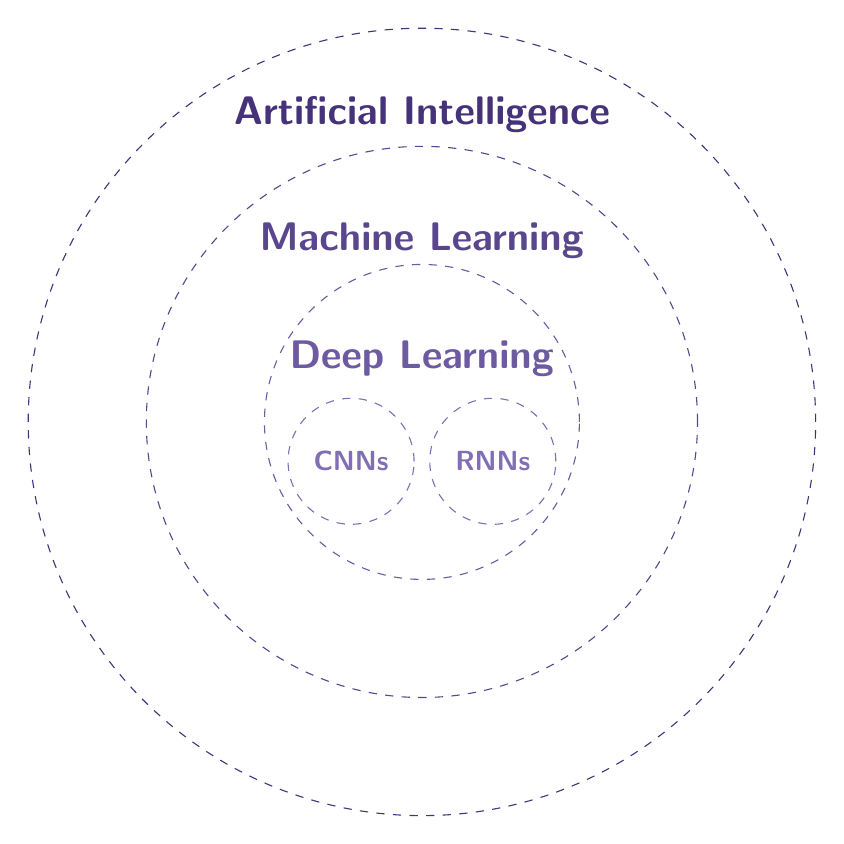
\begin{tikzpicture}[font=\sffamily]
    % Define colors
    \definecolor{outercolor}{RGB}{70,50,120}
    \definecolor{middlecolor}{RGB}{90,70,140}
    \definecolor{innercolor}{RGB}{110,90,160}
    \definecolor{innermostcolor}{RGB}{130,110,180}

    % Outer circle (Artificial Intelligence)
    \draw[dashed, outercolor] (0,0) circle (5cm);
    \node[outercolor] at (0,3.9) {\Large\textbf{Artificial Intelligence}};

    % Middle circle (Machine Learning)
    \draw[dashed, middlecolor] (0,0) circle (3.5cm);
    \node[middlecolor] at (0,2.3) {\Large\textbf{Machine Learning}};

    % Inner circle (Deep Learning)
    \draw[dashed, innercolor] (0,0) circle (2cm);
    \node[innercolor] at (0,0.8) {\Large\textbf{Deep Learning}};

    % Innermost circle (RNNs)
    \draw[dashed, innermostcolor] (-0.9,-0.5) circle (0.8cm);
    \node[innermostcolor] at (-0.9,-0.5) {\textbf{CNNs}};

    \draw[dashed, innermostcolor] (0.9,-0.5) circle (0.8cm);
    \node[innermostcolor] at (0.9,-0.5) {\textbf{RNNs}};

\end{tikzpicture}
\caption{Zusammenhang von Machine Learning, neuronalen Netzen, Deep Learning, \glspl{CNN} und \glspl{RNN}}
\label{fig:ml-hierarchy}
\end{figure}

\subsection{Neuronale Netze}
\label{subsec:neuronale-netze}
Neuronale Netze sind eine Klasse von \gls{ML}-Modellen, die von der Funktionsweise des menschlichen Gehirns inspiriert sind \cite{RebalaGopinath2019AItM}. Sie bestehen aus miteinander verbundenen Neuronen, die in Schichten angeordnet sind:
\begin{itemize}
    \item Eingabeschicht (Input Layer): Nimmt die Eingabedaten auf
    \item Versteckte Schichten (Hidden Layer): Verarbeiten die Informationen
    \item Ausgabeschicht (Output Layer): Liefert das Ergebnis
\end{itemize}

Die Verbindungen zwischen den Neuronen haben Gewichte, die während des Trainings angepasst werden. Durch nichtlineare Aktivierungsfunktionen können neuronale Netze komplexe Zusammenhänge modellieren.

\subsubsection{Deep Learning}
\label{subsec:deep-learning}
Deep learning bezeichnet neuronale Netze die über viele versteckte Schichten verfügen \cite{RebalaGopinath2019AItM}, wodurch hierarchische Merkmale aus den Daten extrahiert werden können. Die Entwicklung von Deep Learning Algorithem führte in den letzten Jahren zu großen Fortschritten im Bereichen wie Bilderkennung, Sprachverarbeitung, Robotik oder auch \gls{OCR}.

\subsubsection{Convolutional Neural Networks (CNNs)}
\label{subsubsec:cnn}


\section{Natural Language Processing (NLP)}
\label{sec:nlp}

\subsection{Tokenisierung}
\label{subsec:tokenisierung}

\subsection{Part-of-Speech Tagging}
\label{subsec:pos-tagging}

\subsection{Named Entity Recognition}
\label{subsec:ner}

\section{Transformer-Architekturen und Large Language Models}
\label{sec:transformers-llms}

\subsection{Transformer-Architektur}
\label{subsec:transformer-architecture}

\subsection{BERT und verwandte Modelle}
\label{subsec:bert}

\subsection{Large Language Models (LLMs)}
\label{subsec:llms}

\subsubsection{LLAMA}
\label{subsubsec:LLAMA}

\subsection{Herausforderungen und Einschränkungen}
\label{subsec:llm-challenges}

\section{Evaluation und Metriken}
\label{sec:evaluation-metrics}

\subsection{Precision, Recall und F1-Score}
\label{subsec:precision-recall-f1}

\subsection{Micro-F1 und Macro-F1}
\label{subsec:micro-macro-f1}

\section{Lernparadigmen und Aufgabenkategorien}
\label{sec:lernparadigmen-aufgabenkategorien}

\subsection{Transfer Learning}
\label{subsec:transfer-learning}

\subsection{Few-Shot Learning}
\label{subsec:few-shot-learning}

\subsection{Zero-Shot Learning}
\label{subsec:zero-shot-learning}

\subsection{Meta-Learning}
\label{subsec:meta-learning}

\subsection{Multitask Learning}
\label{subsec:multitask-learning}
